
\section{Interazione con OBP}
\label{sec:OBP}

L'interfaccia di OBP è una interfaccia RESTful\footnote{L'interfaccia di OBP, in realtà, è in sola lettura. Estendiamo il suo funzionamento anche alla scrittura (inserimento di informazioni nel back-end), poiché l'estensione delle sue funzionalità in questo senso è, almeno logicamente, immediata.}, in cui i dati vengono trasmessi in formato json, e l'autenticazione è gestita tramite protocollo OAuth (versione 1.0, prima revisione) \cite{oauthrfc}.

\subsection{OAuth}

Il protocollo OAuth si basa sul modello client/server, e permette al client di accedere ad una risorsa protetta situata sul server e di propriet\`a di una terza entit\`a senza che questa (detta ``proprietario della risorsa'') debba condividere le proprie credenziali di accesso al server con il client.

\subsubsection{Ruoli}

In OBP i ruoli sono ripartiti nel seguente modo:
\begin{description}
	\item[Client] un'applicazione di terze parti che desideri accedere in lettura o in scrittura ai conti correnti presso la filiale (come il sistema HBS);
	\item[Server] l'API di OBP (e il back-end della banca soggiacente);
	\item[Resource owner] un correntista presso la banca iscritto a HBS;
	\item[Protected resource] un conto corrente di un correntista presso la banca;
	\item[Credentials] le credenziali di accesso alla banca del correntista;
	\item[Token] identificativo univoco fornito dal server al client.
\end{description}
L'applicazione (Client nel gergo di OAuth) possiede a sua volta un token univoco, previsto dallo standard, utilizzato per identificare il Client fra le richieste.

\subsubsection{Token}

In HBS il token per l'accesso ad un account del back-end della banca viene creato alla registrazione dell'utente, e associato all'account HBS del cliente.
La procedura per l'ottenimento del token \`e illustrata in figura \ref{fig:oauth:token}.

\begin{figure*}[h]
    \centering
	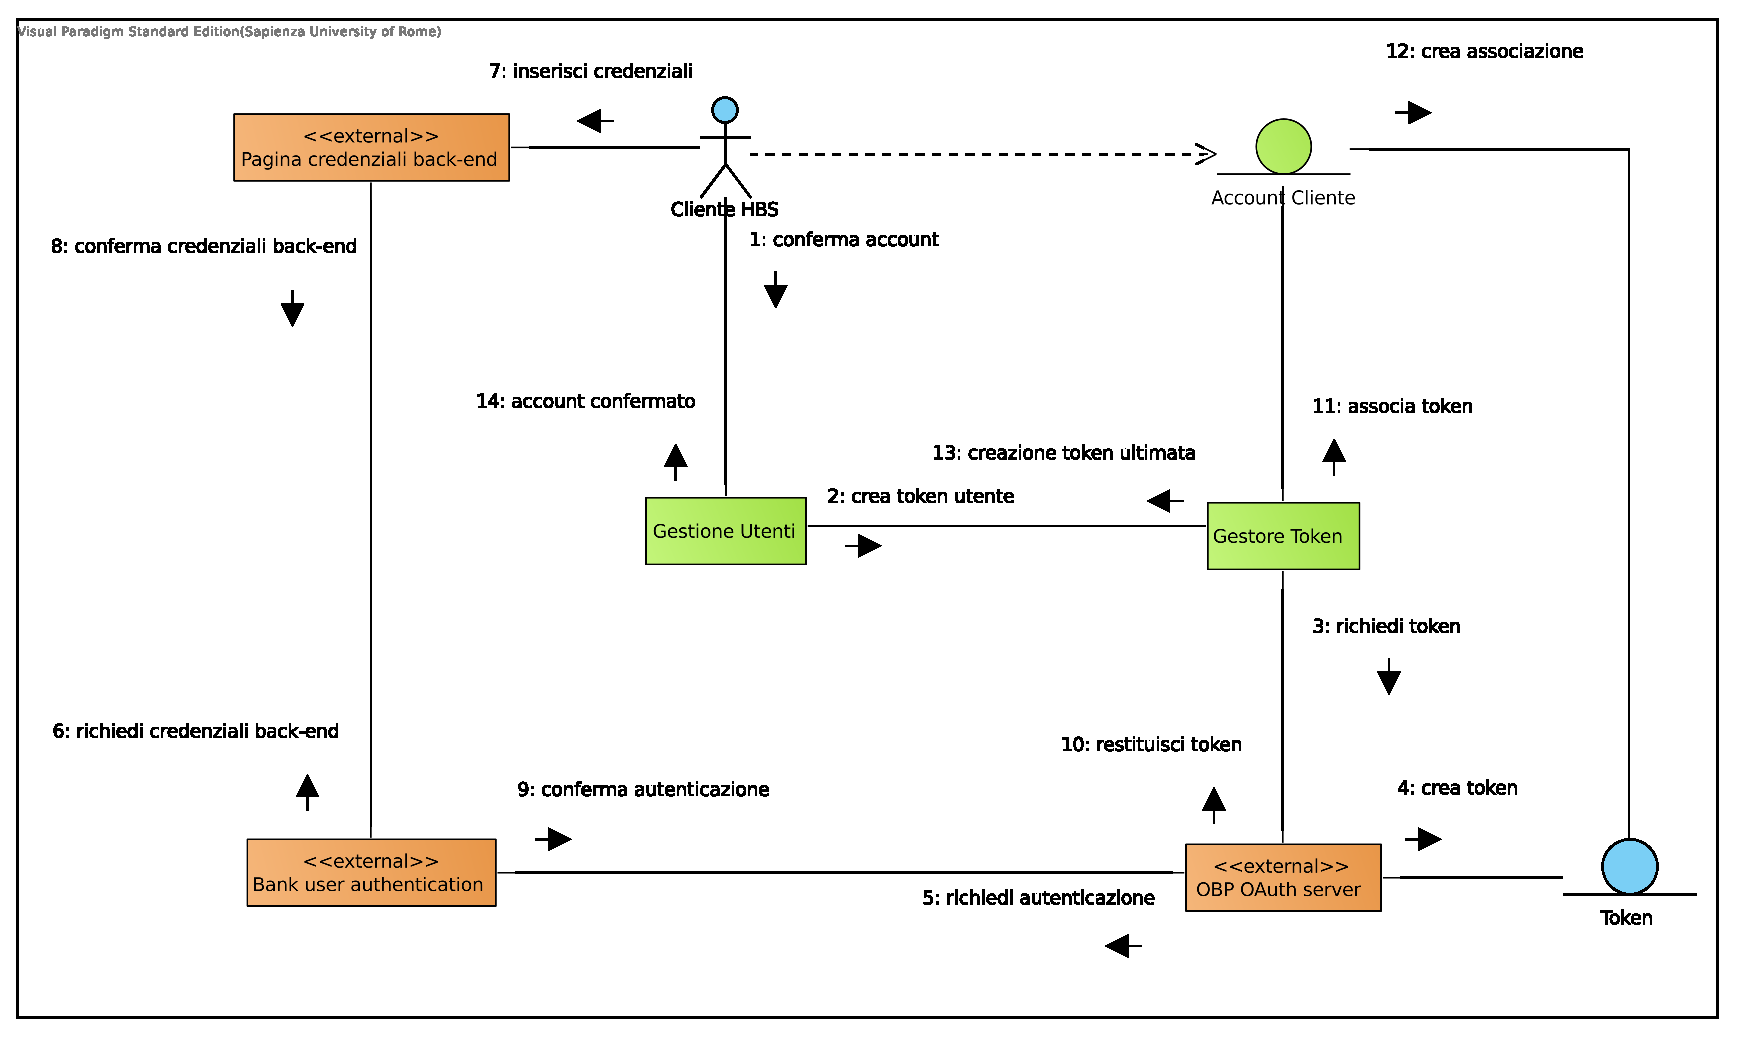
\includegraphics[width=\textwidth]{Images/Ottenimento_Token.eps}
    \caption{Diagramma di comunicazione illustrante la procedura per l'ottenimento del token.}
    \label{fig:oauth:token}
\end{figure*}

HBS ottiene, al momento dell'installazione presso l'istituto, un suo token, utilizzato durante lo scambio di informazioni per l'ottenimento del token di un cliente.

\subsection{Comunicazione}

La procedura per effettuare operazioni (ovvero per inserire una transazione nel back-end della banca, ad esempio) o per effettuare query consiste nell'invio di una richiesta \code{POST} o \code{GET} al server OBP della banca.
Le richieste a OBP condividono tipicamente la stessa struttura dell'header, con qualche differenza nei casi di query pi\`u complesse.
Comune a tutte le richieste sono il token cliente di cui sopra e le chiavi di HBS relative all'istituto.

\begin{figure*}[h]
\begin{lstlisting}[basicstyle=\ttfamily]
POST /accounts/[ACCOUNT_ID]/transactions HTTP/1.1
Host: [indirizzo istituto bancario]
Authorization: OAuth
oauth_token="[token cliente]",
oauth_consumer_key="[chiave istituto bancario]",
oauth_nonce="[nonce]",
oauth_signature="[signature]",
oauth_signature_method="HMAC-SHA256",
oauth_timestamp="[timestamp]",
oauth_version="1.0"

{
    "this_account": {
        "id": [id account],
        "number": [numero conto],
        "IBAN": [iban conto],
        "swift_bic": [codice swift],
        "bank": {
            "national_identifier": [identificatore banca],
            "name": [nome banca]
        }
    },
    "other_account": {
        "holder": {
            "name": [nome beneficiario]
        },
        "number": [numero conto beneficiario],
        "IBAN": [iban beneficiario],
        "swift_bic": [codice swift],
        "bank": {
            "national_identifier": [identificatore istituto beneficiario],
            "name": [nome istituto beneficiario]
        },
    },
    "details": {
        "posted_by_user_id": [id utente],
        "posted_by_ip_address": [ip terminale],
        "type": "cash",
        "description": [causale],
        "posted": [data esecuzione],
        "value": {
            "currency": [valuta],
            "amount": [cifra]
        }
    }
}
\end{lstlisting}
	\caption{\label{fig:operazioni:bonifico-internazionale:json}Inserimento di un bonifico internazionale nel back-end della banca tramite OBP}
\end{figure*}

\subsubsection{Bonifici}

Il messaggio per l'esecuzione di un generico bonifico internazionale \`e mostrato in figura \ref{fig:operazioni:bonifico-internazionale:json}.
Il messaggio viene inviato al server OBP della banca con una richiesta \code{POST}.
Il messaggio di risposta contiene informazioni riguardo l'avvenuta presa in carico dell'operazione da parte del back-end della banca, codificate a loro volta in Json.
La struttura del messaggio \`e simile alla struttura dei messaggi per l'esecuzione di bonifici SEPA, bonifici SEPA italia, etc.: la differenza principale consiste nell'assenza di alcuni campi.

\subsubsection{Query: Saldo e Storico Operazioni}

Raccogliere informazioni riguardo lo stato del conto corrente di un cliente, come ad es.\ il saldo attuale, o le operazioni effettuate in un certo intervallo di tempo, avviene con una richiesta \code{GET}.

Per ottenere il saldo di un conto la struttura della richiesta \`e la seguente:
\begin{lstlisting}[basicstyle=\ttfamily]
GET /accounts/[ACCOUNT_ID]/[VIEW_ID]/account HTTP/1.1
Host: [indirizzo istituto bancario]
Authorization: OAuth
oauth_token="[token cliente]",
oauth_consumer_key="[chiave istituto bancario]",
oauth_nonce="[nonce]",
oauth_signature="[signature]",
oauth_signature_method="HMAC-SHA256",
oauth_timestamp="[timestamp]",
oauth_version="1.0"
\end{lstlisting}
Il messaggio di risposta contiene informazioni riguardanti l'account dell'utente codificate in un array Json.
Il saldo si trova sotto la voce \code{balance}.

L'elenco delle transazioni effettuate da un conto corrente \`e ottenibile a sua volta con una richiesta \code{GET}.
La struttura della richiesta \`e la seguente:
\begin{lstlisting}[basicstyle=\ttfamily]
GET /accounts/[ACCOUNT_ID]/[VIEW_ID]/transactions HTTP/1.1
Host: [indirizzo istituto bancario]
Authorization: OAuth
obp_limit="[numero elementi risposta]"
obp_offset="[offset primo elemento]"
obp_from_date="[data minima]"
obp_to_date="[data massima]"
oauth_token="[token cliente]",
oauth_consumer_key="[chiave istituto bancario]",
oauth_nonce="[nonce]",
oauth_signature="[signature]",
oauth_signature_method="HMAC-SHA256",
oauth_timestamp="[timestamp]",
oauth_version="1.0"
\end{lstlisting}
La richiesta presenta parametri extra nell'header rispetto alle altre richieste, il cui scopo \`e permettere di restringere il periodo di riferimento delle operazioni.


